\documentclass{article}
\usepackage{graphicx} 
\usepackage{dirtytalk}
\usepackage{amsmath}
\usepackage{lmodern}
\usepackage{booktabs}
\usepackage{siunitx}
\usepackage{float}
\usepackage{siunitx}
\usepackage{placeins}
\usepackage{xcolor}

\usepackage[ngerman]{babel}
\usepackage[a4paper, total={6in, 8in}]{geometry}
\begin{document}
\begin{titlepage}
    \begin{center}
        \vspace*{1cm}
            
        \Huge
        \textbf{Auswertung}\\
        Teilversuch 1 und Teilversuch 3 (Korrektur vom 03.03.2026) 
        \vspace{0.5cm}
        \LARGE
        
        
        \vspace{1.8cm}
            
        \textbf{Jonas Müther \& Alejandro Schultheiss} \\
        \vfill
            
        P1 Praktikum\\
       
            
        \vspace{0.8cm}
  

        \vspace{1.8cm}
        \Large
        LMU München \\
        Physik B.Sc.\\
        Deutschland\\
        2026
            
    \end{center}
\end{titlepage}
\tableofcontents

\newpage
\section{Auswertung Teilversuch 1}
\subsection{Flugweite der 3 Kugeln}
Im Folgenden betrachten wir die Flugweite dreier Kugeln mit 3 unterschiedlichen Materialien. Kugel 1 besteht aus Stahl, Kugel 2 aus Glas (Murmel), und Kugel 3 aus Plastik. Die drei Kugeln wurden einzeln unter reproduzierbaren Anfangsbedingungen entlang der Beschleunigungsschiene freigesetzt. Nach Verlassen der Schiene erfolgte eine Übergangsbewegung in den waagerechten Wurf. Die Auftreffpunkte wurden auf einem Transparentpapier registriert, unter dem eine Kohleplatte zur präzisen Markierung positioniert war. Der Versuch wurde für jede Kugel mehrfach wiederholt, bis eine Bestimmung des mittleren Auftrefforts per Augenmaß, möglich war. \\
Die folgenden 3 Tabellen zeigen die Flugweiten für jede der 3 Kugeln: 

\begin{table}[h]
    \centering
    \caption{Gemessene Flugweiten für Stahlkugel (Kugel 1)}
    \vspace{.2cm}
    \label{tab:flugweiten1}
    \begin{tabular}{lc}
        \toprule
        \textbf{Messung} & \textbf{Flugweite} \\
        \midrule
        Flugweite 1 & 28{,}1\,cm \\
        Flugweite 2 & 28{,}2\,cm \\
        Flugweite 3 & 28{,}4\,cm \\
        Flugweite 4 & 28{,}6\,cm \\
        Flugweite 5 & 28{,}7\,cm \\
        \bottomrule
    \end{tabular}
\end{table}

\begin{table}[h]
    \centering
    \caption{Gemessene Flugweiten für Plastikkugel (Kugel 2)}
    \vspace{.2cm}
    \label{tab:flugweiten2}
    \begin{tabular}{lc}
        \toprule
        \textbf{Messung} & \textbf{Flugweite} \\
        \midrule
        Flugweite 1  & 27{,}5\,cm \\
        Flugweite 2  & 27{,}1\,cm \\
        Flugweite 3  & 26{,}4\,cm \\
        Flugweite 4  & 27{,}4\,cm \\
        Flugweite 5  & 27{,}5\,cm \\
        Flugweite 6  & 27{,}2\,cm \\
        Flugweite 7  & 24{,}2\,cm \\
        Flugweite 8  & 27{,}9\,cm \\
        Flugweite 9  & 27{,}9\,cm \\
        Flugweite 10 & 28{,}7\,cm \\
        Flugweite 11 & 28{,}9\,cm \\
        Flugweite 12 & 30{,}3\,cm \\
        Flugweite 13 & 29{,}5\,cm \\
        Flugweite 14 & 29{,}6\,cm \\
        Flugweite 15 & 28{,}2\,cm \\
        Flugweite 16 & 28{,}6\,cm \\
        Flugweite 17 & 30{,}3\,cm \\
        Flugweite 18 & 33{,}8\,cm \\
        \bottomrule
    \end{tabular}
\end{table}

\begin{table}[htpb]
    \centering
    \caption{Gemessene Flugweiten für Glaskugel (Murmel) (Kugel 3)}
    \vspace{.2cm}
    \label{tab:flugweiten3}
    \begin{tabular}{lc}
        \toprule
        \textbf{Messung} & \textbf{Flugweite} \\
        \midrule
        Flugweite 1  & 26{,}9\,cm \\
        Flugweite 2  & 27{,}1\,cm \\
        Flugweite 3  & 27{,}6\,cm \\
        Flugweite 4  & 27{,}8\,cm \\
        Flugweite 5  & 27{,}9\,cm \\
        Flugweite 6  & 28{,}9\,cm \\
        Flugweite 7  & 30{,}2\,cm \\
        Flugweite 8  & 28{,}2\,cm \\
        Flugweite 9  & 28{,}0\,cm \\
        Flugweite 10 & 27{,}9\,cm \\
        Flugweite 11 & 28{,}1\,cm \\
        Flugweite 12 & 25{,}9\,cm \\
        Flugweite 13 & 32{,}1\,cm \\
        Flugweite 14 & 33{,}5\,cm \\
        \bottomrule
    \end{tabular}
\end{table}

\FloatBarrier

\noindent Für sämtliche Messpunkte wird eine globale Ortsunsicherheit angesetzt und in der Fehlerfortpflanzung berücksichtigt: (s. 1.1.1)
\[
    \Delta x = \pm 2\,\mathrm{mm} = \pm 0.2\,\mathrm{cm}.
\]

\noindent\textbf{Bemerkung:} Die Anzahl der gemessenen Flugweiten variiert zwischen den einzelnen Kugeln, 
da nach Augenmaß bestimmt wurde, wann ein mittlerer Auftreffort hinreichend genau erkennbar ist.


\subsubsection{Fehlerdiskussion für das Messen der Flugweiten}
Zur Bestimmung der Flugweiten wurde eine digitale Messmethode eingesetzt, die eine von der direkten Linealmessung abweichende Unsicherheitsstruktur aufweist. Die Methodik, sowie die zugehörigen Unsicherheiten werden nachfolgend erläutert. 
\noindent Um die Flugweiten zu messen, wurde das Transparentpapier eingescannt, wobei zuvor noch die Länge des Papiers mit einem Lineal gemessen wurde. Anschliessend wurde der Scan in ein Vektorbasiertes Grafikprogramm importiert, wobei der Scan im Grafikprogramm auf die zuvor gemessene Länge skaliert wurde. Die anschliessende Bestimmung der Flugweiten erfolgte dann über einzelnd eingezeichnete Linien. (s. Abb. 1) 

\begin{figure}[htbp]
    \centering
    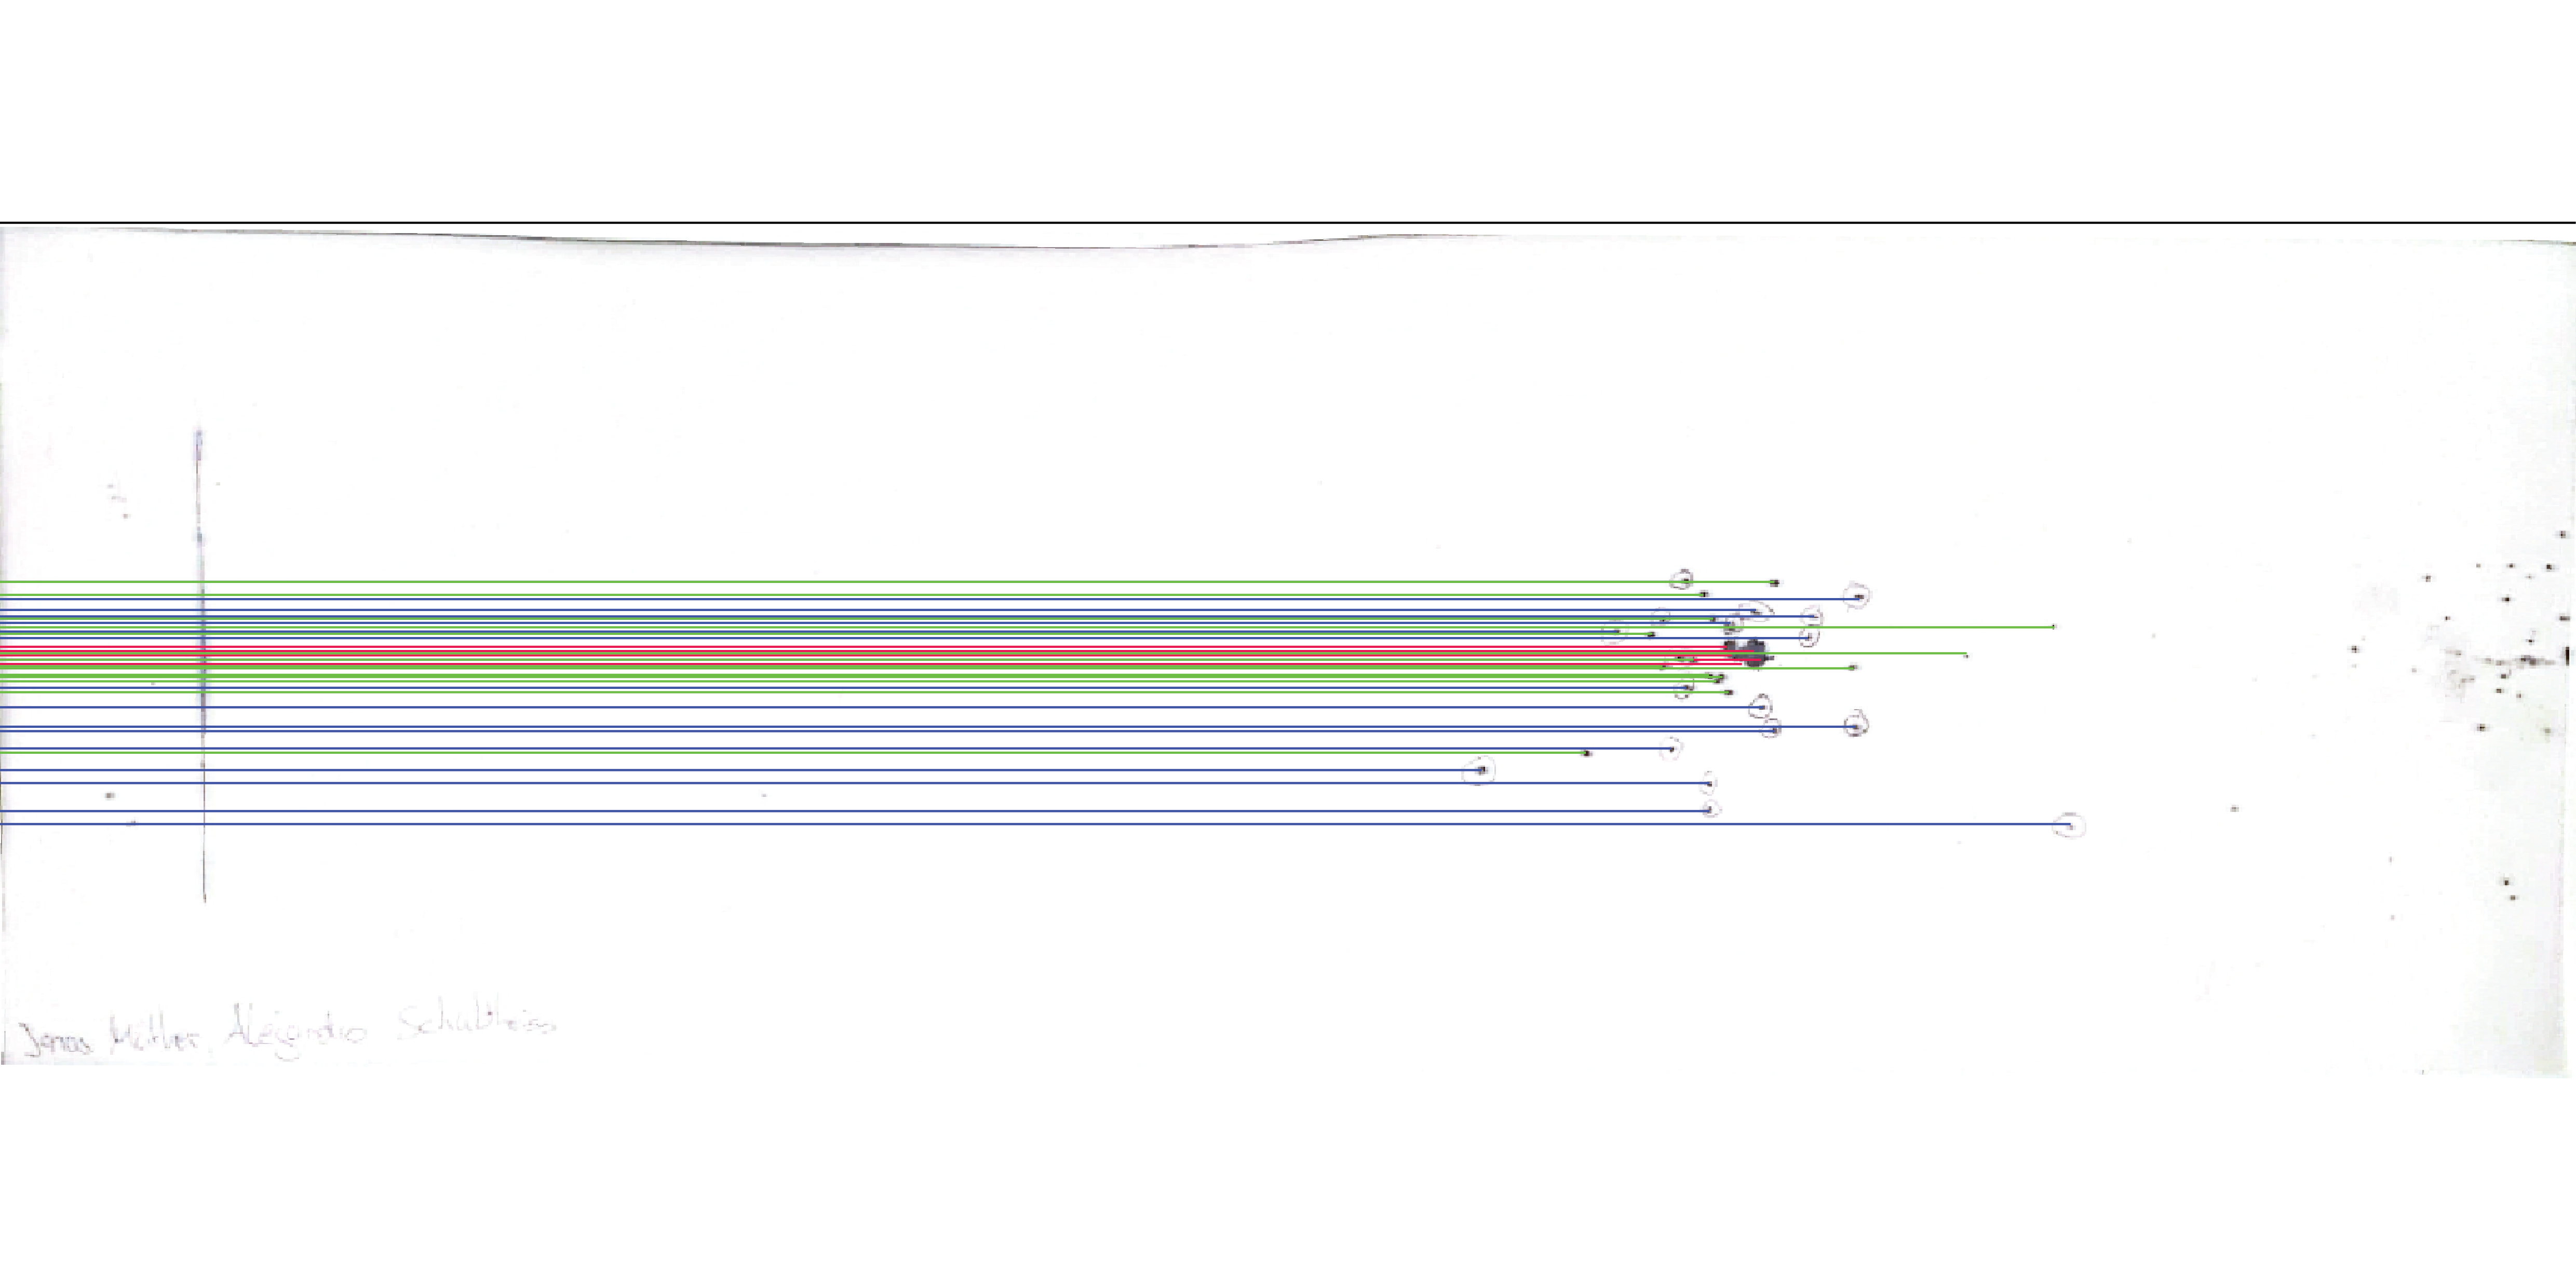
\includegraphics[width=0.7\textwidth]{Images/p1_auswertung_flugweite.png}
    \caption{Flugweitenmessung über digital eingezeichnete Linien}
    \label{fig:beispiel}
\end{figure}

\FloatBarrier


\noindent Folgende Fehlerquellen des Messprozesses wurden dabei in betracht gezogen und abgeschätzt:


\begin{itemize}
    \item \textbf{Punktbestimmung (Fleckdurchmesser $d \approx 1\,\mathrm{mm}$):}\\
    Es wurde die Annahme getroffen, dass jeder Auftreffort einem Punkt gleicht, dies ist in der Realität nicht der Fall. Der maximale Fehler ergibt sich aus der falschen Annahme, dass sich das physikalische Ereignis im Zentrum abspielt, aber in der Realität am Rand stattfindet. Aufgrundessen ergibt sich für diese Art von Fehler:
    \[
        \Delta x_{\text{Punkt}} \approx \frac{d}{2} \approx 0.5\,\mathrm{mm}.
    \]

    \item \textbf{Menschlicher Einfluss (Cursor/Setzen/Ablesen):}\\
    Abschätzung:
    \[
        \Delta x_{\text{human}} \approx 0.5\,\mathrm{mm}.
    \]

    \item \textbf{Kalibrierung/Scan (Skalierung über $42\,\mathrm{cm}$, Wölbung des Papiers / Sonstige Verzerrungen):}\\
    Abschätzung:
    \[
        \Delta x_{\text{kal}} \approx 1.5\,\mathrm{mm}.
    \]
\end{itemize}

\noindent Die Gesamtunsicherheit ergibt sich aus quadratischer Addition:
\[
    \Delta x_{\text{ges}}
    =
    \sqrt{
        (\Delta x_{\text{Punkt}})^2
        +
        (\Delta x_{\text{human}})^2
        +
        (\Delta x_{\text{kal}})^2
    }.
\]

\noindent Einsetzen liefert:
\[
    \Delta x_{\text{ges}}
    =
    \sqrt{
        (0.5\,\mathrm{mm})^2
        +
        (0.5\,\mathrm{mm})^2
        +
        (1.5\,\mathrm{mm})^2
    }
    =
    \sqrt{0.25 + 0.25 + 2.25}\,\mathrm{mm}
    =
    \sqrt{2.75}\,\mathrm{mm}
    \approx 1.66\,\mathrm{mm}.
\]


\[
    \Delta x = \pm 2\,\mathrm{mm} = \pm 0.2\,\mathrm{cm}.
\]





\noindent\textbf{Bemerkung:} Aufgrund der eingeschränkten Verfügbarkeit des Original-Transparentpapiers wurde die Auswertung mittels eines Scans digital durchgeführt.



\subsection{Bestimmung der experimentellen Flugweite und Fehler}
\subsubsection{Stahlkugel (Kugel 1)}

Als experimentelle Flugweite wird der Mittelwert der Messreihe verwendet (s. Tabelle 1). $x_i$ ist dabei die Flugweite $i$:
\[
\bar{x}=\frac{1}{n}\sum_{i=1}^{n}x_i
      =\frac{1}{5}\left(28{,}1+28{,}2+28{,}4+28{,}6+28{,}7\right)\,\mathrm{cm}.
\]

\[
\bar{x}=\frac{1}{5}\left(113{,}3+28{,}7\right)\,\mathrm{cm}
      =\frac{142{,}0}{5}\,\mathrm{cm}
      =28{,}4\,\mathrm{cm}.
\]


\noindent 
Die Flugweite ergibt sich aus dem Abstand zwischen dem \emph{Fußpunkt des Schienenendes} (Nullpunkt) und dem \emph{Auftreffpunkt} der Kugel. 
Der Fehler setzt sich daher aus zwei Beiträgen zusammen: 
(i) der Unsicherheit bei der Einzeichnung des Fußpunkts mit dem Stift (Strichbreite/Setzen) und 
(ii) der Unsicherheit bei der Bestimmung des Auftreffzentrums aufgrund des endlichen Fleckdurchmessers.

\noindent Für den Fleckdurchmesser wird näherungsweise \(d \approx 2\,\mathrm{mm}\) angenommen, sodass das Zentrum etwa auf
\[
\Delta x_{\text{Fleck}} \approx \frac{d}{2} \approx 1\,\mathrm{mm}
\]
bestimmbar ist. 
Die Einzeichnung des Fußpunkts mit dem Stift wird mit
\[
\Delta x_{\text{Fuß}} \approx 1{,}5\,\mathrm{mm}
\]
angesetzt. 
Beide Beiträge werden quadratisch kombiniert:
\[
\Delta x
=
\sqrt{(\Delta x_{\text{Fleck}})^2+(\Delta x_{\text{Fuß}})^2}
=
\sqrt{(1\,\mathrm{mm})^2+(1{,}5\,\mathrm{mm})^2}
\approx 1{,}9\,\mathrm{mm}.
\]
Gerundet ergibt sich damit:
\[
\Delta x \approx \pm 1{,}9\,\mathrm{mm} \approx \pm 0{,}19\,\mathrm{cm}.
\]

\noindent Damit lautet das Ergebnis:
\[
    x_{\mathrm{exp}} = (28{,}40 \pm 0{,}19)\,\si{cm}.
\]


\subsubsection{Plastikkugel (Kugel 2)}

Als experimentelle Flugweite wird der Mittelwert der Messreihe verwendet (s. Tabelle~2). $x_i$ ist dabei die Flugweite $i$:
\[
\bar{x}=\frac{1}{n}\sum_{i=1}^{n}x_i =\frac{1}{18}\left(243{,}1+267{,}9\right)\,\mathrm{cm}
=\frac{511{,}0}{18}\,\mathrm{cm}
=28{,}39\,\mathrm{cm}.
\]

\noindent
Der Fehler berechnet sich analog zu (1.2.1):

\noindent Für den Fleckdurchmesser wird näherungsweise \(d \approx 1\,\mathrm{mm}\) angenommen, sodass das Zentrum etwa auf
\[
\Delta x_{\text{Fleck}} \approx \frac{d}{2} \approx 0{,}5\,\mathrm{mm}
\]
bestimmbar ist.
Die Einzeichnung des Fußpunkts mit dem Stift wird mit
\[
\Delta x_{\text{Fuß}} \approx 1{,}5\,\mathrm{mm}
\]
angesetzt.
Beide Beiträge werden quadratisch kombiniert:
\[
\Delta x
=
\sqrt{(\Delta x_{\text{Fleck}})^2+(\Delta x_{\text{Fuß}})^2}
=
\sqrt{(0{,}5\,\mathrm{mm})^2+(1{,}5\,\mathrm{mm})^2}
\approx 1{,}6\,\mathrm{mm}.
\]
Damit ergibt sich:
\[
\Delta x \approx \pm 1{,}6\,\mathrm{mm} \approx \pm 0{,}16\,\mathrm{cm}.
\]

\noindent Damit lautet das Ergebnis:
\[
x_{\mathrm{exp}} = (28{,}39 \pm 0{,}16)\,\si{cm}.
\]

\subsubsection{Glaskugel (Murmel) (Kugel 3)}

Als experimentelle Flugweite wird der Mittelwert der Messreihe verwendet (s. Tabelle~3). $x_i$ ist dabei die Flugweite $i$:
\[
\bar{x}=\frac{1}{n}\sum_{i=1}^{n}x_i
=\frac{1}{14}\left(196{,}4+203{,}7\right)\,\mathrm{cm}
=\frac{400{,}1}{14}\,\mathrm{cm}
=28{,}58\,\mathrm{cm}.
\]

\noindent
Der Fehler berechnet sich analog zu (1.2.1):

\noindent Für den Fleckdurchmesser wird näherungsweise \(d \approx 1\,\mathrm{mm}\) angenommen, sodass das Zentrum etwa auf
\[
\Delta x_{\text{Fleck}} \approx \frac{d}{2} \approx 0{,}5\,\mathrm{mm}
\]
bestimmbar ist.
Die Einzeichnung des Fußpunkts mit dem Stift wird mit
\[
\Delta x_{\text{Fuß}} \approx 1{,}5\,\mathrm{mm}
\]
angesetzt.
Beide Beiträge werden quadratisch kombiniert:
\[
\Delta x
=
\sqrt{(\Delta x_{\text{Fleck}})^2+(\Delta x_{\text{Fuß}})^2}
=
\sqrt{(0{,}5\,\mathrm{mm})^2+(1{,}5\,\mathrm{mm})^2}
\approx 1{,}6\,\mathrm{mm}.
\]
Damit ergibt sich:
\[
\Delta x \approx \pm 1{,}6\,\mathrm{mm} \approx \pm 0{,}16\,\mathrm{cm}.
\]

\noindent Damit lautet das Ergebnis:
\[
x_{\mathrm{exp}} = (28{,}58 \pm 0{,}16)\,\si{cm}.
\]



\subsection{Korrektur mit Standardabweichung}

Für die Auswertung wird neben dem Ablesefehler auch die Streuung der Messwerte berücksichtigt. 
Dazu werden für jede Kugel der Mittelwert
\[
\bar{x}=\frac{1}{n}\sum_{i=1}^{n}x_i
\]
und die Standardabweichung
\[
s=\sqrt{\frac{1}{n-1}\sum_{i=1}^{n}(x_i-\bar{x})^2}
\]
berechnet. 

Der statistische Fehler des Mittelwerts ist
\[
\Delta x_{\mathrm{stat}}=\frac{s}{\sqrt{n}}.
\]

Mit dem bereits bestimmten Ablesefehler ergibt sich der Gesamtfehler zu
\[
\Delta x=\sqrt{(\Delta x_{\mathrm{abl}})^2+(\Delta x_{\mathrm{stat}})^2}.
\]

\subsection*{Stahlkugel (Kugel 1)}
Für die Stahlkugel wurden \(n=5\) Messwerte aufgenommen:
\[
28{,}1;\;28{,}2;\;28{,}4;\;28{,}6;\;28{,}7\;\mathrm{cm}.
\]

Der Mittelwert beträgt:
\[
\bar{x}_{\mathrm{Stahl}}=\frac{28{,}1+28{,}2+28{,}4+28{,}6+28{,}7}{5}
=28{,}40\,\mathrm{cm}.
\]

Die Standardabweichung ergibt:
\[
s_{\mathrm{Stahl}}=0{,}255\,\mathrm{cm}.
\]

Damit folgt für den statistischen Fehler des Mittelwerts:
\[
\Delta x_{\mathrm{stat,Stahl}}
=\frac{0{,}255}{\sqrt{5}}
=0{,}114\,\mathrm{cm}.
\]

Für die Stahlkugel wurde der Ablesefehler bereits zu
\[
\Delta x_{\mathrm{abl,Stahl}}=0{,}19\,\mathrm{cm}
\]
bestimmt.

Der Gesamtfehler ist somit:
\[
\Delta x_{\mathrm{Stahl}}
=\sqrt{(0{,}19)^2+(0{,}114)^2}\,\mathrm{cm}
=0{,}222\,\mathrm{cm}.
\]

Damit lautet das Ergebnis:
\[
x_{\mathrm{exp,Stahl}}=(28{,}40\pm0{,}22)\,\mathrm{cm}.
\]

\subsection*{Plastikkugel (Kugel 2)}
Für die Plastikkugel wurden \(n=18\) Messwerte aufgenommen:
\[
27{,}5;\;27{,}1;\;26{,}4;\;27{,}4;\;27{,}5;\;27{,}2;\;24{,}2;\;27{,}9;\;27{,}9;\;28{,}7;\;28{,}9;\;30{,}3;\;29{,}5;\;29{,}6;\;28{,}2;\;28{,}6;\;30{,}3;\;33{,}8\;\mathrm{cm}.
\]

Der Mittelwert beträgt:
\[
\bar{x}_{\mathrm{Plastik}}
=\frac{1}{18}\sum_{i=1}^{18}x_i
=28{,}39\,\mathrm{cm}.
\]

Die Standardabweichung ergibt:
\[
s_{\mathrm{Plastik}}=1{,}990\,\mathrm{cm}.
\]

Damit folgt für den statistischen Fehler des Mittelwerts:
\[
\Delta x_{\mathrm{stat,Plastik}}
=\frac{1{,}990}{\sqrt{18}}
=0{,}469\,\mathrm{cm}.
\]

Für die Plastikkugel wird der bereits bestimmte Ablesefehler
\[
\Delta x_{\mathrm{abl,Plastik}}=0{,}16\,\mathrm{cm}
\]
verwendet.

Der Gesamtfehler ist somit:
\[
\Delta x_{\mathrm{Plastik}}
=\sqrt{(0{,}16)^2+(0{,}469)^2}\,\mathrm{cm}
=0{,}496\,\mathrm{cm}.
\]

Damit lautet das Ergebnis:
\[
x_{\mathrm{exp,Plastik}}=(28{,}39\pm0{,}50)\,\mathrm{cm}.
\]

\subsection*{Glaskugel (Kugel 3)}
Für die Glaskugel wurden \(n=14\) Messwerte aufgenommen:
\[
26{,}9;\;27{,}1;\;27{,}6;\;27{,}8;\;27{,}9;\;28{,}9;\;30{,}2;\;28{,}2;\;28{,}0;\;27{,}9;\;28{,}1;\;25{,}9;\;32{,}1;\;33{,}5\;\mathrm{cm}.
\]

Der Mittelwert beträgt:
\[
\bar{x}_{\mathrm{Glas}}
=\frac{1}{14}\sum_{i=1}^{14}x_i
=\frac{400{,}1}{14}\,\mathrm{cm}
=28{,}58\,\mathrm{cm}.
\]

Die Standardabweichung ergibt:
\[
s_{\mathrm{Glas}}=2{,}052\,\mathrm{cm}.
\]

Damit folgt für den statistischen Fehler des Mittelwerts:
\[
\Delta x_{\mathrm{stat,Glas}}
=\frac{2{,}052}{\sqrt{14}}
=0{,}548\,\mathrm{cm}.
\]

Für die Glaskugel wird der bereits bestimmte Ablesefehler
\[
\Delta x_{\mathrm{abl,Glas}}=0{,}16\,\mathrm{cm}
\]
verwendet.

Der Gesamtfehler ist somit:
\[
\Delta x_{\mathrm{Glas}}
=\sqrt{(0{,}16)^2+(0{,}548)^2}\,\mathrm{cm}
=0{,}571\,\mathrm{cm}.
\]

Damit lautet das Ergebnis:
\[
x_{\mathrm{exp,Glas}}=(28{,}58\pm0{,}57)\,\mathrm{cm}.
\]












\subsection{Mittlerer Auftreffpunkt \& Fehlerkreis}
\subsubsection{Grafische Bestimmung des Fehlerkreises}

Für jede Kugelart wird zunächst der mittlere Auftreffpunkt als Zentrum des Fehlerkreises festgelegt. 
Hierzu wird der experimentelle Mittelwert \(\bar{x}\) der Flugweiten als Mittelpunkt auf der Auftreffebene eingetragen. 
Der Radius \(r\) des Fehlerkreises wird anschließend grafisch so gewählt, dass etwa \(\frac{2}{3}\) der gemessenen Auftreffpunkte innerhalb des Kreises liegen. 
Dazu wird ein Kreis mit Mittelpunkt \(\bar{x}\) schrittweise vergrößert, bis ungefähr:
\[
m=\frac{2}{3}n
\]
der insgesamt \(n\) Messpunkte vom Kreis eingeschlossen werden.
\subsubsection{Fehlerkreis Stahlkugel (Kugel 1)}

\begin{figure}[htbp]
    \centering
    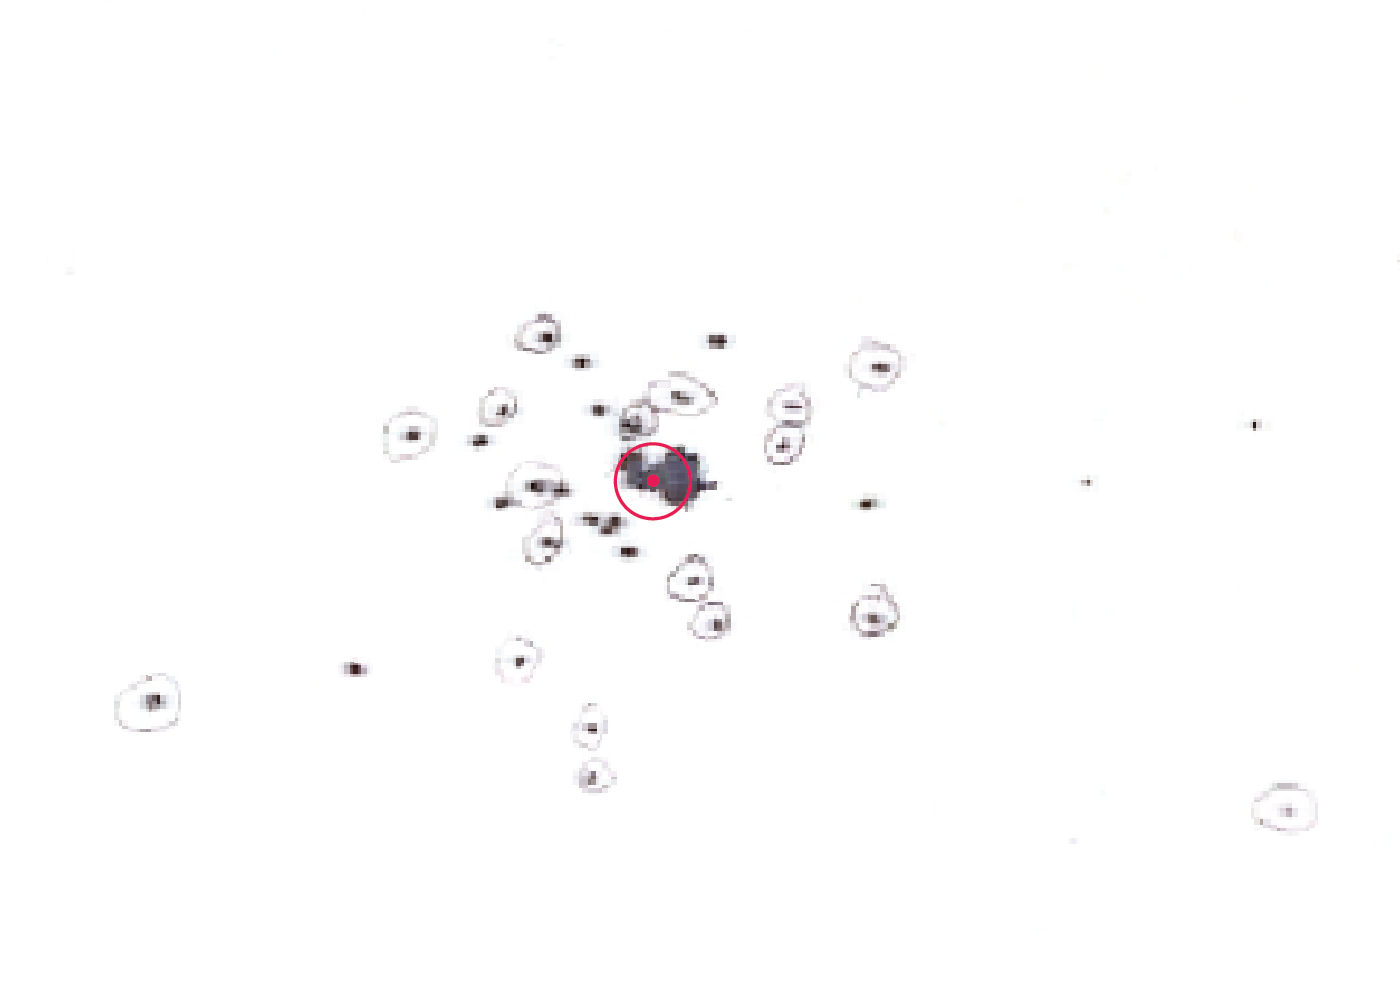
\includegraphics[width=0.7\textwidth]{Images/kugel1.png}
    \caption{Punkt mit Farbe Magenta entspricht dem mittleren Auftrefftpunkt, der Fehlerkreis ist um den Auftreffpunkt zentriert}
    \label{fig:kugel1}
\end{figure}

\FloatBarrier

\subsubsection{Fehlerkreis Plastikkugel (Kugel 2)}
\begin{figure}[htbp]
    \centering
    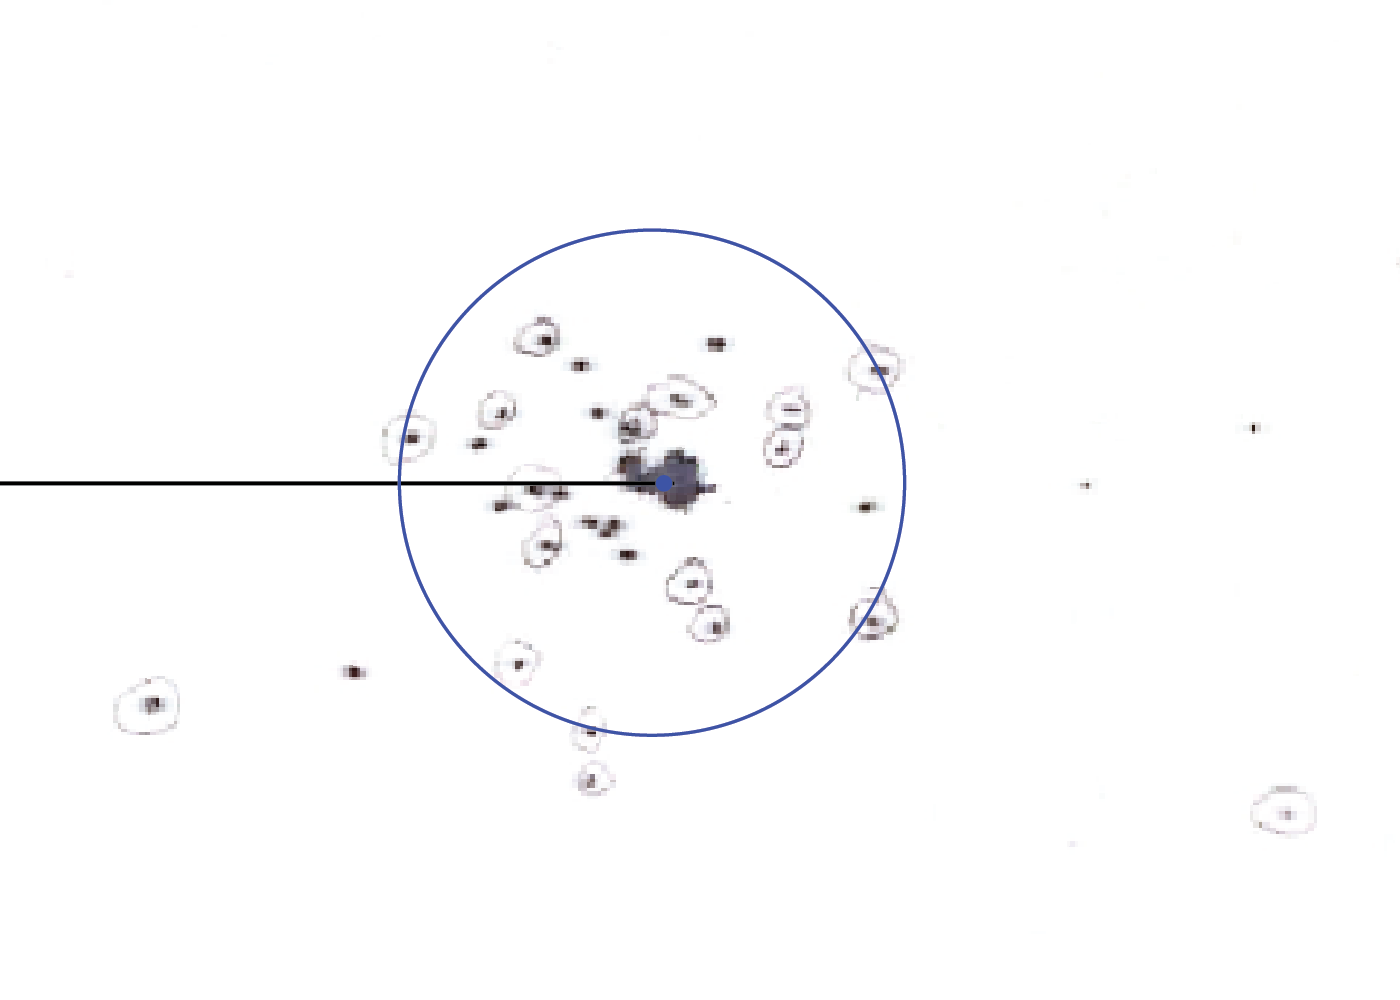
\includegraphics[width=0.7\textwidth]{Images/kugel2.png}
    \caption{Punkt mit Farbe Blau entspricht dem mittleren Auftrefftpunkt, der Fehlerkreis ist um den Auftreffpunkt zentriert}
    \label{fig:kugel2}
\end{figure}



\FloatBarrier

\subsubsection{Fehlerkreis Glaskugel (Kugel 3)}
\begin{figure}[htbp]
    \centering
    \includegraphics[width=0.7\textwidth]{Images/kugel3.png}
    \caption{Punkt mit Farbe Grün entspricht dem mittleren Auftrefftpunkt, der Fehlerkreis ist um den Auftreffpunkt zentriert}
    \label{fig:kugel4}
\end{figure}

\FloatBarrier

\noindent\textbf{Bemerkung:} Ist die Zahl $m$ keine ganze Zahl wird sie aufgerundet. Des weiteren ist zu erwähnen, dass der Fehlerkreis kleiner ist, je weniger die Werte um den Mittelwert streuen, also je konstanter die Flugbahn der Kugel ist. 

\noindent Aufgrund der Rahmenbedingung des mittleren Auftreffpunkts als Mittelpunkt des Fehlerkreises, ist nicht gewährleistet, dass sich jeder Punkt ohne Überschneidung inner- oder außerhalb des Kreises befindet. In so einem Fall, wurde wie folgt abgeschätzt; Wenn beispielsweise 1 Punkt außerhalb des Kreises liegen soll, dies aber ohne Überschneidung nicht möglich ist, da die Punkte zum Beipsiel sehr dicht beieinander liegen, dann
wird aus der Summe der exkludierten Teilflächen mehrerer Punkte,  abgeschätzt wann die Gesamtfläche eines einzigen Punktes erreicht wird. 

\subsection{Berechnung der theoretischen Flugweite der Stahlkugel (Kugel 1)}
\subsubsection{Theoretische Grundlagen}

Anfangs ruht die Kugel auf dem Beschleuniger. Dabei hat sie die Höhe $h1$, und besitzt somit potentielle Energie $Epot$. Beim herunterollen wird diese potentielle Energie $Epot$ in Rotationsenergie $Erot$ und kinetische Energie $Ekin$ umgesetzt.

\begin{figure}[htbp]
    \centering
    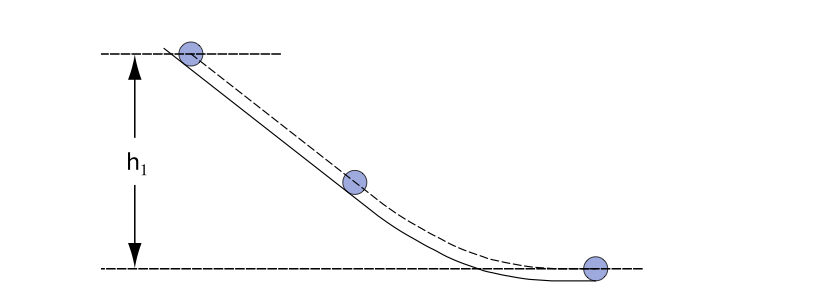
\includegraphics[width=0.7\textwidth]{Images/kugel_start.png}
    \caption{Kugel hat Anfangs Höhe $h1$. \\ Quelle: https://downloads.physik.uni-muenchen.de/praktikum/durst/p1/STO.pdf}
    \label{fig:beschleuniger}
\end{figure}

\FloatBarrier

\noindent In dem System aus Kugel und Beschleuniger lässt sich folgendes Energiegleichgewicht aufstellen:

\begin{equation}
E_{pot} = E_{kin} + E_{rot}
\end{equation}
\begin{equation}
mgh = \frac{1}{2}mv^{2} + \frac{1}{2}I\omega^{2}
\end{equation}

\noindent Das Trägheitsmoment einer Vollkugel sei gegeben durch: 
\begin{equation}
I_{\text{Vollkugel}}=\frac{2}{5}\,mr^{2}\,
\end{equation}

Ferner ist zu beachten, dass sich die Kugel auf einer Schiene bewegt und somit 2 seitliche Kontakpunkte beseitzt. Aus dieser Tatsache folgt, dass die Kugel einen effektiven Rollradius besitzt. 

\begin{figure}[htbp]
    \centering
    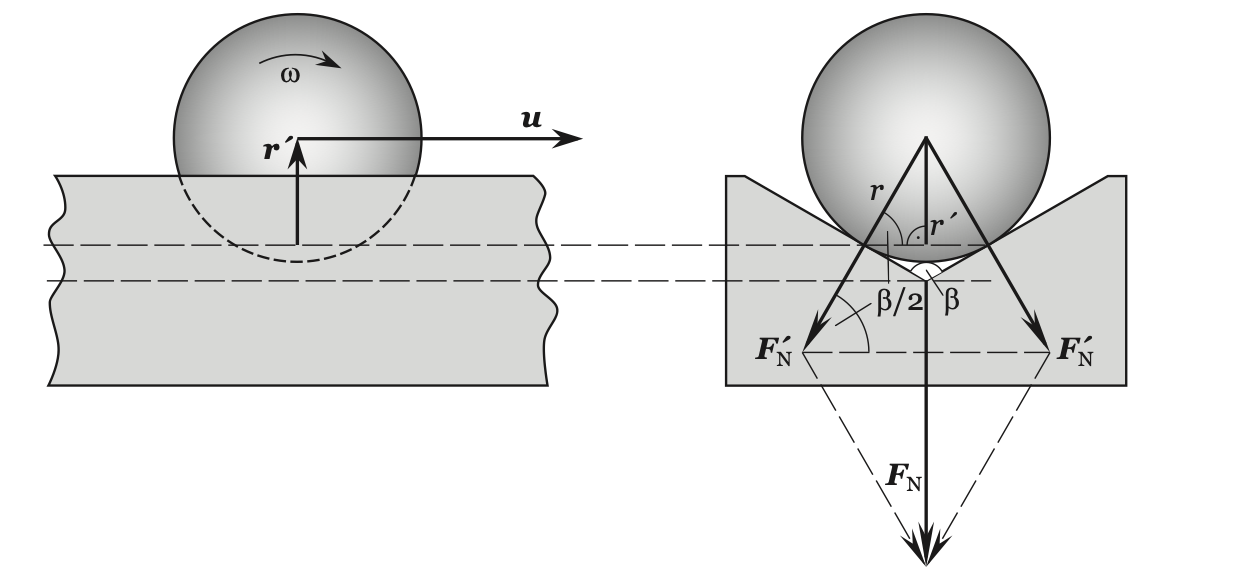
\includegraphics[width=0.7\textwidth]{Images/kugel_auf_schiene.png}
    \caption{Darstellung des effektiven Rollradius $r'$. \\ Quelle: https://downloads.physik.uni-muenchen.de/praktikum/durst/p1/STO.pdf}
    \label{fig:rollradius}
\end{figure}

\FloatBarrier

\noindent Für $r'$ gilt dann, gemäß Skizze und trigonometrischer Funktionen: 

\begin{equation}
r' = r sin(\frac{\beta}{2})
\end{equation}

\noindent
Wir betrachten zudem den Fall des rutschfreien Rollens. Dabei gilt folgende Beziehung zwischen der Translationsgeschwindigkeit $v$ und der Rotationsgeschwindigkeit $\omega$:


\begin{equation}
v = \frac{\mathrm{d}s}{\mathrm{d}t} = r' \frac{\mathrm{d}\phi}{\mathrm{d}t} = r' \omega
\end{equation}

\noindent \textbf{Zur Kenntnisnahme:} Nach dem herunterollen geht die Kugel in einen waagerechten Wurf über. 


\subsubsection{Berechnung der Abfluggeschwindigkeit}
Mit der kurzen Einführung über die theoretischen Grundlagen (1.4.1) der vorliegenden physikalischen Ereignisse, können wir nun die Abfluggeschwindigkeit $v$ berechnen, welche uns im weiteren Verlauf helfen wird die Flugweite zu bestimmen. Wir betrachten eine Kugel mit $d = 20mm$, $r' = rsin\frac{\beta}{2}$, $h1 = 229,0mm$ und einem Winkel $\beta = 120^{\circ}$ und starten mit Gleichung $(1)$ bzw. $(2)$: 

\begin{equation}
mgh_{1} = \frac{1}{2}mv^{2} + \frac{1}{2}I\omega^{2}
\end{equation}

Einsetzen von $(3)$ in $(6)$, liefert:

\begin{equation}
mgh_{1} = \frac{1}{2}mv^{2} + \frac{2}{10}\,mr^{2}\, \omega^{2}
\end{equation}

$(5)$ in $(7)$:

\begin{equation}
mgh_{1} = \frac{1}{2}mv^{2} + \frac{2}{10}\,mr^{2}\, \frac{v^{2}}{r^{2} sin^{2}(\frac{\beta}{2})}
\end{equation}

Kürzen und zusammenfassen liefert:
\begin{equation}
gh_{1} = \frac{1}{2}v^{2} + \frac{1}{5}\,r^{2}\, \frac{v^{2}}{sin^{2}(\frac{\beta}{2})}
\end{equation}

Umformen nach $v$, liefert die geüwnschte Gleichung für die Abfluggeschwindigkeit $v$:

\begin{equation}
v = \sqrt{\frac{2gh_{1}}{1+\frac{2}{5sin^{2}(\frac{\beta}{2})}}}
\end{equation}

\subsubsection{Berechnung der Dauer $t$ des freien Falls}
Nachdem die Kugel in den waagerechten Wurf übergegangen ist, gilt für die vergangene Zeit $t$ in $y$-Richtung:
\begin{equation}
h_{1} = \frac{1}{2}gt^{2}
\end{equation}

\begin{equation}
t = \sqrt{\frac{2h_{1}}{g}}
\end{equation}


\subsubsection{Berechnung der theoretischen Flugweite}
Nun können wir die theoretische Flugweite berechnen. 
Für die zurückgelegte Strecke $x$ in $x$-Richtung beim waagerechten Wurf gilt:

\begin{equation}
x = vt
\end{equation}

$(10), (12)$ in $(13)$ liefet:

\begin{equation}
x = \sqrt{\frac{2gh_{1}}{1+\frac{2}{5sin^{2}(\frac{\beta}{2})}}}\sqrt{\frac{2h_{1}}{g}} = \sqrt{\frac{4gh_{1}^{2}}{(1+\frac{2}{5sin^{2}(\frac{\beta}{2})})g}}
\end{equation}

Einsetzen bekannter Werte liefert für die Flugweite $x$:

\begin{equation}
x = \sqrt{\frac{4gh_{1}^{2}}{(1+\frac{2}{5sin^{2}(\frac{\beta}{2})})g}}
\end{equation}

% Gegeben:
% β = 120^\circ, \quad h_1 = 229.0\,\mathrm{mm} = 0.2290\,\mathrm{m}, \quad
% g = 9.807\,\mathrm{m\,s^{-2}} \ \text{(fehlerfrei)}
%
% Vollkugel: I = \frac{2}{5}mR^2

\begin{equation}
x
= \sqrt{\frac{4 g h_{1}^{2}}{\left(1+\frac{2}{5\sin^{2}\!\left(\frac{\beta}{2}\right)}\right)g}}
= \sqrt{\frac{4 h_{1}^{2}}{1+\frac{2}{5\sin^{2}\!\left(\frac{\beta}{2}\right)}}}
= \frac{2h_1}{\sqrt{1+\frac{2}{5\sin^{2}\!\left(\frac{\beta}{2}\right)}}}\,.
\end{equation}

\begin{align}
\sin^{2}\!\left(\frac{\beta}{2}\right)
&= \sin^{2}(60^\circ)
= \left(\frac{\sqrt{3}}{2}\right)^{2}
= \frac{3}{4},\\[4pt]
1+\frac{2}{5\sin^{2}\!\left(\frac{\beta}{2}\right)}
&= 1+\frac{2}{5\cdot \frac{3}{4}}
= 1+\frac{2}{\frac{15}{4}}
= 1+\frac{8}{15}
= \frac{23}{15}.
\end{align}

\begin{equation}
x
= \frac{2h_1}{\sqrt{23/15}}
= 2h_1\sqrt{\frac{15}{23}}
\stackrel{h_1=0.2290\,\mathrm{m}}{=}
2\cdot 0.2290\,\mathrm{m}\,\sqrt{\frac{15}{23}}
\approx 0.3699\,\mathrm{m}
= 369.9\,\mathrm{mm}.
\end{equation}

\vspace{.5cm}
Für die gaußsche Fehlerfortpflanzung gilt:
\begin{equation}
\sigma_x
= \sqrt{\left(\frac{\partial x}{\partial h_1}\sigma_{h_1}\right)^2
      +\left(\frac{\partial x}{\partial \beta}\sigma_{\beta}\right)^2
      +\left(\frac{\partial x}{\partial g}\sigma_{g}\right)^2}\,.
\end{equation}

% Partielle Ableitungen:
\begin{align}
\frac{\partial x}{\partial h_1}
&= \frac{2}{\sqrt{1+\frac{2}{5\sin^{2}\!\left(\frac{\beta}{2}\right)}}},\\[6pt]
\frac{\partial x}{\partial \beta}
&= -\,h_1\left(1+\frac{2}{5\sin^{2}\!\left(\frac{\beta}{2}\right)}\right)^{-\frac{3}{2}}
\cdot \frac{\mathrm{d}}{\mathrm{d}\beta}\!\left(\frac{2}{5\sin^{2}\!\left(\frac{\beta}{2}\right)}\right),\\[6pt]
\frac{\partial x}{\partial g}
&= 0
\qquad\text{(da sich $g$ in der gegebenen Formel herauskürzt).}
\end{align}

% Da laut Aufgabenstellung β, h1 und g als fehlerfrei anzunehmen sind:
\begin{equation}
\sigma_{h_1}=0,\qquad \sigma_{\beta}=0,\qquad \sigma_{g}=0
\quad\Longrightarrow\quad
\sigma_x = 0.
\end{equation}


\paragraph{Üebereinstimmung innerhalb der Fehler.}
Da gemäß Aufgabenstellung $\beta$, $h_1$ und $g$ als fehlerfrei anzunehmen sind,
ist die theoretische Unsicherheit (Gau{\ss}-Fortpflanzung) null:
\begin{equation}
\sigma_{x,\mathrm{theo}}
= \sqrt{\left(\frac{\partial x}{\partial h_1}\sigma_{h_1}\right)^2
      +\left(\frac{\partial x}{\partial \beta}\sigma_{\beta}\right)^2
      +\left(\frac{\partial x}{\partial g}\sigma_{g}\right)^2}
=0
\qquad(\sigma_{h_1}=\sigma_\beta=\sigma_g=0).
\end{equation}
Die Abweichung und deren Unsicherheit lauten somit
\begin{equation}
\Delta x = x_\mathrm{exp}-x_\mathrm{theo},
\qquad
\sigma_{\Delta x}=\sqrt{\sigma_{x,\mathrm{exp}}^2+\sigma_{x,\mathrm{theo}}^2}
=\sigma_{x,\mathrm{exp}}.
\end{equation}
Numerisch ergibt sich
\begin{equation}
\Delta x = 28.4\,\mathrm{cm}-36.99\,\mathrm{cm}=-8.59\,\mathrm{cm},
\qquad
|\Delta x|=8.59\,\mathrm{cm},
\qquad
\sigma_{\Delta x}=0.19\,\mathrm{cm}.
\end{equation}
Damit gilt
\begin{equation}
|\Delta x| = 8.59\,\mathrm{cm} \gg 0.19\,\mathrm{cm}=\sigma_{\Delta x},
\end{equation}
also stimmen experimenteller und theoretischer Wert nicht innerhalb der Fehler überein.

\paragraph{Rückrechnung der effektiven Fallhoehe}
Um zu prüfen, ob eine falsch eingesetzte Fallhöhe $h_1$ die Diskrepanz erklären kann,
wird die Formel nach $h_1$ umgestellt:
\begin{equation}
x = 2h_1\sqrt{\frac{15}{23}}
\quad\Longrightarrow\quad
h_1 = \frac{x}{2}\sqrt{\frac{23}{15}}.
\end{equation}
Setzt man den experimentellen Mittelwert $x_\mathrm{exp}=28.0\,\mathrm{cm}=0.280\,\mathrm{m}$ ein, folgt
\begin{equation}
h_{1,\mathrm{eff}}
= \frac{0.280\,\mathrm{m}}{2}\sqrt{\frac{23}{15}}
\approx 0.173\,\mathrm{m}
=173\,\mathrm{mm}.
\end{equation}
Verglichen mit der verwendeten Hoehe $h_1=229\,\mathrm{mm}$ ergibt sich eine Differenz von
\begin{equation}
\Delta h_1 = 229\,\mathrm{mm}-173\,\mathrm{mm}=56\,\mathrm{mm}.
\end{equation}

\noindent
Eine Abweichung solcher Größenordnung, lässt sich nicht allein durch physikalische Phänomene wie Reibung o.ä. erklären. In der Berechnung muss mir ein Fehler unterlaufen sein. Anderweitig wäre noch ein plausibles Argument, dass die Startvorrichtung nicht perfekt am höchsten Punkt sitzt und so dem Projektil ca. 5cm an Höhe fehlen. 



\subsection{Korrektur: Nutzung der korrekten Formel STO - (15)}



\textcolor{red}{Achtung: Uns ist aufgefallen, dass beim digitalen ablesen der Flugweiten ein Fehler nicht berücksichtigt wurde. Die genaue Fehlerquelle ist schwer zu bestimmen und kann nur angenommen werden. Es ist davon auszugehen, dass es dabei nicht nur einen einzigen Fehler gibt, sondern eine ganze Reihe an Fehlerquellen. Folge davon ist, dass in dieser Auswertung mit eine experimentellen Flugweite von $\approx 28cm$ (digital gemessen) gerechnet wurde; die experimentelle Flugweite sich aber analog gemessen (Lineal) auf $\approx 23cm$ beläfut. Daraus lässt sich schliessen, wie bereits vermutet, dass sich beim digitalen ablesen ein großer Gesamtfehler eingeschlichten hat. Mögliche Fehlerquellen sind dabei: Wölbung des Papiers, Ungenauer Scan, digital falsch skaliert, ungenaues ablesen, uä. Für die Zukunft gilt diese ganzen Zwischenschritte zu vermeiden und eine Messemethode zu wählen, die so wenig Zwischenschritte wie möglich besitzt, da sich so der Gesamtfehler reduziert. Aus diesem Grund ist z.b.: der Reibungskoeffizent negativ, was physiklisch keinen Sinn ergibt. Die folgenden Korrekturen und Rechnungen sollten trotzdem korrekt sein.}




% --- Gegeben (Stahlkugel, d = 20 mm) ---
% beta = 120^\circ  (fehlerfrei)
% h_1  = 229.0 mm = 0.2290 m (fehlerfrei)
% g    = 9.807 m/s^2 (fehlerfrei)
%
% Bestimmung der Fallhöhe:
% H = (Boden bis höchster Punkt der Kugel) = 138 mm mit Abweichung 1 mm
% d = Kugeldurchmesser = (20.00 \pm 0.03) mm
% => h_2 = H - d

\subsubsection*{Bestimmung der Fallhöhe \(h_2\) inklusive Unsicherheit}
Die Fallhöhe ergibt sich aus der gemessenen Gesamthöhe \(H\) (Boden bis höchster Punkt der Kugel)
abzüglich des Kugeldurchmessers \(d\):
\begin{equation}
h_2 = H - d.
\end{equation}
Mit
\begin{equation}
H = (138 \pm 1)\,\mathrm{mm}, \qquad d = (20.00 \pm 0.03)\,\mathrm{mm}
\end{equation}
folgt
\begin{equation}
h_2 = 138\,\mathrm{mm} - 20.00\,\mathrm{mm} = 118.0\,\mathrm{mm}.
\end{equation}

Da \(H\) und \(d\) unabhängig sind, ergibt sich die Unsicherheit von \(h_2\) über Gauß:
\begin{equation}
\sigma_{h_2} =
\sqrt{\left(\frac{\partial h_2}{\partial H}\sigma_H\right)^2
     +\left(\frac{\partial h_2}{\partial d}\sigma_d\right)^2}
=
\sqrt{(1\cdot\sigma_H)^2 + ((-1)\cdot\sigma_d)^2}
=
\sqrt{\sigma_H^2+\sigma_d^2}.
\end{equation}
Damit
\begin{equation}
\sigma_{h_2}=\sqrt{(1\,\mathrm{mm})^2+(0.03\,\mathrm{mm})^2}
\approx 1.00\,\mathrm{mm}.
\end{equation}

\subsubsection*{Theoretische Flugweite \(x_{\mathrm{theo}}\) (STO-(15))}
Die theoretische Flugweite lautet
\begin{equation}
x_{\mathrm{theo}}
=\sqrt{\frac{4h_1h_2}{1+\frac{2}{5\sin^2\!\left(\frac{\beta}{2}\right)}}}.
\end{equation}

Für \(\beta=120^\circ\) gilt
\begin{align}
\sin^{2}\!\left(\frac{\beta}{2}\right)
&=\sin^{2}(60^\circ)=\frac{3}{4},\\[4pt]
D \;:=\; 1+\frac{2}{5\sin^{2}\!\left(\frac{\beta}{2}\right)}
&=1+\frac{2}{5\cdot\frac{3}{4}}
=\frac{23}{15}.
\end{align}

Mit \(h_1=0.2290\,\mathrm{m}\) und \(h_2=0.1180\,\mathrm{m}\) folgt
\begin{equation}
x_{\mathrm{theo}}
=\sqrt{\frac{4\cdot 0.2290\,\mathrm{m}\cdot 0.1180\,\mathrm{m}}{23/15}}
\approx 0.26550\,\mathrm{m}
= 26.55\,\mathrm{cm}.
\end{equation}

\subsubsection*{Gaußsche Fehlerfortpflanzung für \(x_{\mathrm{theo}}\)}
Allgemein gilt
\begin{equation}
\sigma_{x,\mathrm{theo}}
= \sqrt{\left(\frac{\partial x}{\partial h_1}\sigma_{h_1}\right)^2
      +\left(\frac{\partial x}{\partial h_2}\sigma_{h_2}\right)^2
      +\left(\frac{\partial x}{\partial \beta}\sigma_{\beta}\right)^2
      +\left(\frac{\partial x}{\partial g}\sigma_{g}\right)^2}\,.
\end{equation}
Da sich \(g\) in \(x_{\mathrm{theo}}\) herauskürzt, ist \(\frac{\partial x}{\partial g}=0\).
Gemäß Aufgabenstellung sind \(\beta\), \(h_1\) und \(g\) fehlerfrei:
\begin{equation}
\sigma_{h_1}=0,\qquad \sigma_{\beta}=0,\qquad \sigma_{g}=0,
\end{equation}
wobei \(h_2\) \emph{nicht} fehlerfrei ist (\(\sigma_{h_2}\neq 0\)).

Mit \(x=\sqrt{\frac{4h_1h_2}{D}}\) ergibt sich
\begin{equation}
\frac{\partial x}{\partial h_2}
=\frac{2h_1}{D\,x}.
\end{equation}
Damit reduziert sich die theoretische Unsicherheit zu
\begin{equation}
\sigma_{x,\mathrm{theo}}
=
\left|\frac{\partial x}{\partial h_2}\right|\sigma_{h_2}
=
\frac{2h_1}{D\,x_{\mathrm{theo}}}\,\sigma_{h_2}.
\end{equation}

Numerisch (mit \(D=\frac{23}{15}\), \(h_1=0.2290\,\mathrm{m}\), \(x_{\mathrm{theo}}=0.26550\,\mathrm{m}\)):
\begin{equation}
\frac{2h_1}{D\,x_{\mathrm{theo}}}\approx 1.125
\quad\Longrightarrow\quad
\sigma_{x,\mathrm{theo}} \approx 1.125\cdot\sigma_{h_2}.
\end{equation}
Mit \(\sigma_{h_2}\approx 1.00\,\mathrm{mm}=0.10\,\mathrm{cm}\) folgt
\begin{equation}
\sigma_{x,\mathrm{theo}} \approx 1.125\cdot 0.10\,\mathrm{cm} \approx 0.11\,\mathrm{cm}.
\end{equation}

\subsubsection*{Übereinstimmung innerhalb der Fehler (Stahlkugel)}
Experimentell (korrigiert):
\begin{equation}
x_{\mathrm{exp}}=(28.40\pm0.22)\,\mathrm{cm}.
\end{equation}

Abweichung:
\begin{equation}
\Delta x = x_{\mathrm{exp}}-x_{\mathrm{theo}}
= 28.40\,\mathrm{cm}-26.55\,\mathrm{cm}
= 1.85\,\mathrm{cm}.
\end{equation}

Unsicherheit der Abweichung:
\begin{equation}
\sigma_{\Delta x}
=\sqrt{\sigma_{x,\mathrm{exp}}^{2}+\sigma_{x,\mathrm{theo}}^{2}}
=\sqrt{(0.22\,\mathrm{cm})^{2}+(0.11\,\mathrm{cm})^{2}}
\approx 0.25\,\mathrm{cm}.
\end{equation}

Vergleich:
\begin{equation}
|\Delta x| = 1.85\,\mathrm{cm} \gg 0.25\,\mathrm{cm}=\sigma_{\Delta x},
\end{equation}
also stimmen experimenteller und theoretischer Wert nicht innerhalb der Fehler überein.



\subsection{Berechnung des Reibungskoeffizienten}
%------------------------------------------------------------
% Aufgabe: Bestimmen Sie den Reibungskoeffizienten \kappa und seinen Fehler.
% Gegeben: S = 728\,mm (fehlerfrei),
%          h_1 = 229.0\,mm (fehlerfrei),
%          s_\mathrm{exp} = (28.0 \pm 0.19)\,cm = (280 \pm 1.9)\,mm,
%          s_\mathrm{theo} = 369.9\,mm (theoretischer Wert, fehlerfrei)
%------------------------------------------------------------

\paragraph{Bestimmung von \texorpdfstring{$\kappa$}{kappa}.}
Aus dem Skript gilt bei rutschfreiem Rollen:
\begin{equation}
\frac{\Delta u^2}{u^2}=\kappa\,\frac{S}{h_1},
\qquad
\frac{\Delta u^2}{u^2}=1-\frac{s_\mathrm{exp}^2}{s_\mathrm{theo}^2}.
\end{equation}
Damit folgt direkt:
\begin{equation}
{\;
\kappa=\frac{h_1}{S}\left(1-\frac{s_\mathrm{exp}^2}{s_\mathrm{theo}^2}\right)
\;}
\end{equation}

\paragraph{Numerischer Wert.}
\begin{equation}
\kappa
=\frac{229.0}{728}\left(1-\frac{280^2}{369.9^2}\right)
\approx 0.1343.
\end{equation}

\paragraph{Fehler nach Gau{\ss} (mit \texorpdfstring{$S$}{S} fehlerfrei).}
Da $S$ als fehlerfrei anzunehmen ist (und hier auch $h_1$ sowie $s_\mathrm{theo}$ als fehlerfrei verwendet werden),
traegt nur die Unsicherheit von $s_\mathrm{exp}$ bei:
\begin{equation}
\sigma_\kappa
=\left|\frac{\partial \kappa}{\partial s_\mathrm{exp}}\right|\sigma_{s_\mathrm{exp}}.
\end{equation}
Mit
\begin{equation}
\kappa(s_\mathrm{exp})=\frac{h_1}{S}\left(1-\frac{s_\mathrm{exp}^2}{s_\mathrm{theo}^2}\right)
\end{equation}
ergibt sich
\begin{equation}
\frac{\partial \kappa}{\partial s_\mathrm{exp}}
=\frac{h_1}{S}\left(-\frac{2s_\mathrm{exp}}{s_\mathrm{theo}^2}\right).
\end{equation}
Also
\begin{equation}
\sigma_\kappa
=\frac{h_1}{S}\,\frac{2s_\mathrm{exp}}{s_\mathrm{theo}^2}\,\sigma_{s_\mathrm{exp}}.
\end{equation}
Mit $\sigma_{s_\mathrm{exp}}=0.19\,\mathrm{cm}=1.9\,\mathrm{mm}$:
\begin{equation}
\sigma_\kappa
=\frac{229.0}{728}\,\frac{2\cdot 280}{369.9^2}\,(1.9)
\approx 2.45\times 10^{-3}.
\end{equation}

\paragraph{Ergebnis:}
\begin{equation}
{\kappa = 0.1343 \pm 0.0024}
\end{equation}

\subsection{Korrektur}
\paragraph{Bestimmung von \texorpdfstring{$\kappa$}{kappa}.}
Aus STO gilt (Energieverlust durch Reibung):
\begin{equation}
\frac{\Delta u^2}{u^2}=\kappa\,\frac{S}{h_1},
\qquad
\frac{\Delta u^2}{u^2}=1-\frac{s_\mathrm{exp}^2}{s_\mathrm{th}^2}.
\end{equation}
Damit folgt
\begin{equation}
\kappa=\frac{h_1}{S}\left(1-\frac{s_\mathrm{exp}^2}{s_\mathrm{th}^2}\right).
\end{equation}

\paragraph{Numerischer Wert.}
Mit
\[
h_1=229.0\,\mathrm{mm},\quad S=728\,\mathrm{mm},\quad
s_\mathrm{exp}=28.40\,\mathrm{cm},\quad s_\mathrm{th}=26.55\,\mathrm{cm}
\]
ergibt sich
\begin{equation}
\kappa
=\frac{229.0}{728}\left(1-\frac{28.40^2}{26.55^2}\right)
\approx -0.0454.
\end{equation}

\paragraph{Fehler nach Gau{\ss} (mit \texorpdfstring{$S$}{S} und \texorpdfstring{$h_1$}{h1} fehlerfrei).}
Da \(S\) und \(h_1\) als fehlerfrei angenommen werden, tragen nur \(s_\mathrm{exp}\) und \(s_\mathrm{th}\) bei:
\begin{equation}
\sigma_\kappa=
\sqrt{
\left(\frac{\partial \kappa}{\partial s_\mathrm{exp}}\sigma_{s_\mathrm{exp}}\right)^2
+
\left(\frac{\partial \kappa}{\partial s_\mathrm{th}}\sigma_{s_\mathrm{th}}\right)^2}.
\end{equation}
Mit
\begin{equation}
\kappa(s_\mathrm{exp},s_\mathrm{th})
=\frac{h_1}{S}\left(1-\frac{s_\mathrm{exp}^2}{s_\mathrm{th}^2}\right)
\end{equation}
folgt
\begin{align}
\frac{\partial \kappa}{\partial s_\mathrm{exp}}
&=
-\frac{h_1}{S}\frac{2s_\mathrm{exp}}{s_\mathrm{th}^2},\\[4pt]
\frac{\partial \kappa}{\partial s_\mathrm{th}}
&=
\frac{h_1}{S}\frac{2s_\mathrm{exp}^2}{s_\mathrm{th}^3}.
\end{align}
Damit
\begin{equation}
\sigma_\kappa=
\sqrt{
\left(\frac{h_1}{S}\frac{2s_\mathrm{exp}}{s_\mathrm{th}^2}\sigma_{s_\mathrm{exp}}\right)^2
+
\left(\frac{h_1}{S}\frac{2s_\mathrm{exp}^2}{s_\mathrm{th}^3}\sigma_{s_\mathrm{th}}\right)^2}.
\end{equation}

\paragraph{Einsetzen.}
Mit \(\sigma_{s_\mathrm{exp}}=0.22\,\mathrm{cm}\) und \(\sigma_{s_\mathrm{th}}=0.11\,\mathrm{cm}\):
\begin{equation}
\sigma_\kappa\approx 0.0063.
\end{equation}

\paragraph{Ergebnis.}
\begin{equation}
\kappa = -0.0454 \pm 0.0063.
\end{equation}

\paragraph{Hinweis zur Interpretation.}
Das negative Vorzeichen entsteht hier, weil \(s_\mathrm{exp}>s_\mathrm{th}\) gilt.
Da \(\kappa\) im Modell als Reibungs-/Verlustparameter eingeführt wird, deutet \(\kappa<0\)
auf eine Inkonsistenz zwischen idealisierter Theorie (STO) und Experiment bzw. auf
systematische Effekte hin. Da die experimentellen Flugweiten digital vom Transparentpapier abgelesen wurden, ist es plausibel, dass eine große Fehlerquelle nicht beachtet wurde (Falsch skaliert, starke Wölbung des Papiers, Scan ungenau, u.ä.). Siehe rot markierten Hinweis.

\newpage
\section{Auswertung Teilversuch 3}
\textbf{Bemerkung}: Teile der Auswertung zu Teilversuch 3, sind bitte dem Praktikumsprotkoll zu entnehmen.

\subsection{Berechnung der theoretisch erwarteten Werte für Beschleunigung und Geschwindigkeit}

%------------------------------------------------------------
% Theoretische Werte: Beschleunigung a (schiefe Ebene) und Abfluggeschwindigkeit u
% Gegeben: \alpha = 37^\circ, \beta = 120^\circ, h_1 = 229.0\,mm = 0.2290\,m,
%          g = 9.807\,m/s^2, Vollkugel: I = (2/5)mR^2
%------------------------------------------------------------

\paragraph{Abfluggeschwindigkeit:}
Es gilt folgende Formel:
\begin{equation}
u
= \sqrt{\frac{2 g h_1}{1+\frac{2}{5\sin^{2}\!\left(\frac{\beta}{2}\right)}}}\,.
\end{equation}
Für $\beta=120^\circ$ gilt:
\begin{equation}
\sin^{2}\!\left(\frac{\beta}{2}\right)=\sin^{2}(60^\circ)=\frac{3}{4},
\qquad
1+\frac{2}{5\sin^{2}\!\left(\frac{\beta}{2}\right)}
=1+\frac{2}{5\cdot\frac{3}{4}}
=\frac{23}{15}.
\end{equation}
Damit:
\begin{equation}
u
=\sqrt{\frac{2 g h_1}{23/15}}
=\sqrt{2 g h_1\,\frac{15}{23}}.
\end{equation}
Mit $g=9.807\,\mathrm{m\,s^{-2}}$ und $h_1=0.2290\,\mathrm{m}$:
\begin{equation}
u
=\sqrt{2\cdot 9.807\cdot 0.2290\cdot \frac{15}{23}}
\approx 1.71\,\mathrm{m\,s^{-1}}.
\end{equation}

\paragraph{Beschleunigung auf der schiefen Ebene}

Für die Beschleunigung gilt:
\begin{equation}
a
= \frac{g\sin\alpha}{1+\frac{2}{5\sin^{2}\!\left(\frac{\beta}{2}\right)}}\,.
\end{equation}
Fuer $\alpha=37^\circ$ und wie oben $\left(1+\frac{2}{5\sin^{2}(\beta/2)}\right)=\frac{23}{15}$ folgt
\begin{equation}
a
= g\sin(37^\circ)\,\frac{15}{23}.
\end{equation}
Numerisch:
\begin{equation}
a
= 9.807\cdot \sin(37^\circ)\cdot \frac{15}{23}
\approx 3.85\,\mathrm{m\,s^{-2}}.
\end{equation}

\paragraph{Ergebnis:}
\begin{equation}
{u \approx 1.71\,\mathrm{m\,s^{-1}},\qquad a \approx 3.85\,\mathrm{m\,s^{-2}}.}
\end{equation}
%------------------------------------------------------------

\subsection{Diskussion der theoretischen und experimentell gemessenen Werte}
%------------------------------------------------------------
% Vergleich Experiment vs. Theorie und Diskussion
%------------------------------------------------------------

\paragraph{Theoriewerte:}
\begin{equation}
g_\mathrm{theo}=9.81\,\mathrm{m\,s^{-2}},\qquad
u_\mathrm{theo}\approx 1.71\,\mathrm{m\,s^{-1}},\qquad
a_\mathrm{theo}\approx 3.85\,\mathrm{m\,s^{-2}}.
\end{equation}

\paragraph{Experimentelle Werte (Analyse):}
\begin{equation}
g_\mathrm{exp}=(9.22\pm 0.02)\,\mathrm{m\,s^{-2}},\qquad
u_\mathrm{exp}=(1.6\pm 0.2)\,\mathrm{m\,s^{-1}},\qquad
a_\mathrm{exp}=(3.886\pm 0.01)\,\mathrm{m\,s^{-2}}.
\end{equation}

\paragraph{Abweichungen.}
\begin{align}
\Delta g &= g_\mathrm{exp}-g_\mathrm{theo} = 9.22-9.81 = -0.59\,\mathrm{m\,s^{-2}},\\
\Delta u &= u_\mathrm{exp}-u_\mathrm{theo} = 1.6-1.71 = -0.11\,\mathrm{m\,s^{-1}},\\
\Delta a &= a_\mathrm{exp}-a_\mathrm{theo} = 3.886-3.85 = +0.036\,\mathrm{m\,s^{-2}}.
\end{align}

\paragraph{Kompatibilitaetscheck (innerhalb der Fehler)}
Unter der Annahme, dass die Theoriewerte fehlerfrei sind, gilt als Kriterium:
\begin{equation}
|\Delta x| \le \sigma_{x,\mathrm{exp}}.
\end{equation}
Damit folgt:
\begin{align}
|\Delta g| &= 0.59\,\mathrm{m\,s^{-2}} \gg 0.02\,\mathrm{m\,s^{-2}}
&&\Rightarrow\ \text{keine Uebereinstimmung},\\
|\Delta u| &= 0.11\,\mathrm{m\,s^{-1}} < 0.2\,\mathrm{m\,s^{-1}}
&&\Rightarrow\ \text{Uebereinstimmung},\\
|\Delta a| &= 0.036\,\mathrm{m\,s^{-2}} > 0.01\,\mathrm{m\,s^{-2}}
&&\Rightarrow\ \text{keine Uebereinstimmung}.
\end{align}

\paragraph{Diskussion möglicher Ursachen:}
Die Abweichung von $u$ ist mit der relativ grossen experimentellen Unsicherheit vereinbar.
Die signifikanten Abweichungen bei $g$ und $a$ deuten dagegen auf systematische Effekte hin,
z.\,B.\ eine nicht exakt bekannte Geometrie (tatsaechlicher Neigungswinkel $\alpha$ weicht vom Herstellerwert ab),
Reibungs- und Rollverluste (nicht ideal rutschfreies Rollen), sowie Messsystematiken
(Zeiterfassung/Trigger für Start Stopp der Highspeedkamera, Ablesefehler bei Strecken, Nullpunkt/Bezug der Höhe). Man beachte, dass der Prozess des Messvorgangs extrem Fehleranfällig ist. Unter dieser Rücksichtsnahme, stellen die Theoriewerte eine gute Näherung dar.

\end{document}
